% This must be in the first 5 lines to tell arXiv to use pdfLaTeX, which is strongly recommended.
\pdfoutput=1
% In particular, the hyperref package requires pdfLaTeX in order to break URLs across lines.

\documentclass[11pt]{article}

% Remove the "review" option to generate the final version.
\usepackage[review]{ACL2023}

% Standard package includes
\usepackage{times}
\usepackage{latexsym}

% For proper rendering and hyphenation of words containing Latin characters (including in bib files)
\usepackage[T1]{fontenc}
% For Vietnamese characters
% \usepackage[T5]{fontenc}
% See https://www.latex-project.org/help/documentation/encguide.pdf for other character sets

% This assumes your files are encoded as UTF8
\usepackage[utf8]{inputenc}

% This is not strictly necessary, and may be commented out.
% However, it will improve the layout of the manuscript,
% and will typically save some space.
\usepackage{microtype}

% This is also not strictly necessary, and may be commented out.
% However, it will improve the aesthetics of text in
% the typewriter font.
\usepackage{inconsolata}

%% Use the graphicx package to include figures.
\usepackage{graphicx}
\usepackage{caption}
\usepackage{subcaption}
\usepackage{placeins}
\usepackage{fancyvrb}
\usepackage{amsmath}

\DeclareMathOperator*{\argmax}{arg\,max}
\DeclareMathOperator*{\argmin}{arg\,min}
% If the title and author information does not fit in the area allocated, uncomment the following
%
%\setlength\titlebox{<dim>}
%
% and set <dim> to something 5cm or larger.

\title{Examining Calibration Large Language Model in Question Answering}

% Author information can be set in various styles:
% For several authors from the same institution:
% \author{Author 1 \and ... \and Author n \\
%         Address line \\ ... \\ Address line}
% if the names do not fit well on one line use
%         Author 1 \\ {\bf Author 2} \\ ... \\ {\bf Author n} \\
% For authors from different institutions:
% \author{Author 1 \\ Address line \\  ... \\ Address line
%         \And  ... \And
%         Author n \\ Address line \\ ... \\ Address line}
% To start a seperate ``row'' of authors use \AND, as in
% \author{Author 1 \\ Address line \\  ... \\ Address line
%         \AND
%         Author 2 \\ Address line \\ ... \\ Address line \And
%         Author 3 \\ Address line \\ ... \\ Address line}

\author{Aakarsh Nair\\
  University of Tuebingen / Geschwister-Scholl-Platz, 72074 Tübingen\\
  \texttt{aakarsh.nair@aakarsh.nair@student.uni-tuebingen.de} 
  Second Author \\
  Affiliation / Address line 1 \\
  Affiliation / Address line 2 \\
  Affiliation / Address line 3 \\
  \texttt{email@domain} \\}

\begin{document}
\maketitle

%% Abstract: Short summary of the paper (up to 150 words), 
%% should include the conclusion of your study.

\begin{abstract}
In this paper, we examine the issue of calibration of large language models. 
That is the relationship between the \emph{confidence} 
of a predicted answer on a question-answering task 
with its \emph{empirical likelihood of being correct}.

We replicate elements of previous calibration study \cite{kadavath2022language} 
on several multiple-choice  (MMLU, LogicQA, TruthfulQA) and 
open-ended question answering datasets translated into 
the multiple choice format (TriviaQA, HumanEval, GSM8k). 

We find that models do scale in their calibration ability by model size. Moreover models fine-tuned as conversation agents do 
improve in their calibration and accuracy under 
few-shot prompting. 

However, we also observe that for tasks beyond models 
reasoning  capability (complex logical and scientific reasoning) 
fine-tuning harms model's accuracy and leads to 
overconfidence in model predictions.

\end{abstract}


\section{Introduction}

%% Introduction: Introduction, Motivation and explanation of
%% the research question in the \emph{context of the field}/the 
%% class, explaining why it is interesting/novel in 
%% comparison to extant related work. Note that it is NOT 
%% mandatory to include an exhaustive literature review; 
%% it is sufficient to mention relevant work from the project 
%% proposals and the class materials.

Understanding the reliability and correctness of language model (LM) generations is crucial in ensuring their practical utility and trustworthiness. One significant aspect of this inquiry pertains to the calibration of LMs and their ability to accurately indicate uncertainty about their outputs. This issue has gathered considerable attention in recent research, particularly within the context of large-scale language models.

In the paper, Kadavath et al. [2022], it extensively examined the calibration of big base LMs, demonstrating their well-calibrated nature. Their study revealed that the probabilities assigned to answer options on benchmark datasets such as BIGBench and MMLU correlated effectively with the correctness probabilities across trials. However, investigations into reinforcement learning-based language models (RL-LMs) have raised concerns about calibration deterioration following fine-tuning [OpenAI, 2023; Kadavath et al., 2022], albeit with inconsistent findings.

Moreover, an additional challenge in LM-generated content relates to the occurrence of hallucinations, where the model generates false or improbable information. To address this, fine-tuning LMs with reinforcement learning has been suggested, with the goal of prompting responses like "I don't know" to receive high rewards. However, concerns have been raised regarding the potential evasiveness of such models. The present project seeks to provide more comprehensive understanding and explore various aspects of calibration in RL-LMs.



\section{Methods}

%% Methods: Detailed description of the study addressing the 
%% research question (including all details of, e.g., 
%% the models, datasets, used analyses, etc...). 
%% It should enable another person reading your paper to *fully*
%% replicate the study. *No results* or *interpretation* 
%% should be included yet.

\subsection{Introduction}
%% TODO: Not enough mathematical explanation of what the term mean. 
%% TODO: Not explaining, what log completion probbilty means. 
%% TODO: No explantation of transfoerm completion. 

We measure the calibration in keeping with the methodology 
presented in \cite{kadavath2022language}. 

\subsection{Inference Datasets}

In order to understand the the behavior of base vs fine-tuned chat models (models fine tuned as conversational agents). We test out models of varying sizes (7b, 13b and in some cases 70b parameters) on a variety of question answering datasets. A brief explanation of the datasets used is given here:

\subsubsection{MMLU}

The Measuring Massive Multitask Language Understanding (MMLU) 
\cite{hendryckstest2021} \cite{hendrycks2021ethics} is a massive dataset of multiple choice questions which covers 57 tasks in various subjects including elementary mathematics, US history, computer science, law, and more. For convenience the datasets are grouped into 
four categories \emph{STEM},  \emph{Humanities}, \emph{Social Sciences}, and \emph{Other}(global facts, marketing, accounting etc.). Questions test the model for both factual and conceptual understanding of the given topics.

\subsubsection{LogicQA}

LogicQA \cite{liu2020logiqa} is a comprehensive dataset, which is sourced from expert-written questions for testing human logical reasoning. It consists of 8,678 QA instances, covering multiple types of deductive reasoning. Neural modes still lag human performance 
on these questions.

\subsubsection{TruthfulQA}

TruthfulQA \cite{lin2021truthfulqa} is a benchmark to measure whether 
a language model is truthful in generating answers to questions. The benchmark comprises 817 questions that span 38 categories, including health, law, finance and politics. Questions are crafted so that some humans would answer falsely due to a false belief or misconception. To perform well, models must avoid generating false answers learned from imitating human texts.  

\subsubsection{TrivaiQA}

\subsubsection{HumanEval}

\subsubsection{GSM8k}

GSM8K (Grade School Math 8K) is a dataset of 8.5K high quality linguistically diverse grade school math word problems. The dataset was created to support the task of question answering on basic mathematical problems that require multi-step reasoning.

These problems take between 2 and 8 steps to solve. Solutions primarily involve performing a sequence of elementary calculations using basic arithmetic operations  to reach the final answer. A bright middle school student should be able to solve every problem: from the paper, "Problems require no concepts beyond the level of early Algebra, and the vast majority of problems can be solved without explicitly defining a variable." Solutions are provided in natural language, as opposed to pure math expressions. 

\subsection{Multiple Choice Query Format}

MMLU, LogicQA and TruthfulQA datasets provide a set of options for each
question in their dataset along with the most appropriate answer. The choices provided are converted are multiple choice question format with lettered set of options next to each possible answer followed by the answer prompt. A sample question prompt might look like: 

\begin{figure}
\begin{Verbatim}
This question refers to the following 
information.

To him I shall come when I go beyond this 
life, and to him will come he who has faith 
and doubts not.
—The Upanishads, India, c. 1000 BCE

To which religion does the speaker most 
likely belong?

(A). Hinduism
(B). Buddhism
(C). Shintoism
(D). Zoroastrianism

Answer:
\end{Verbatim}
\caption{Sample Question from MMLU Dataset}
\end{figure}

Constraining the model generation to one of these options 
allows us to judge the relative probability of each the answer completions by looking at the token completion probability 
for each of the  formatted options $(A),(B) \dots (D)$ 
respectively. In a few shot example we include multiple questions 
with the answer completion filled in after the prompt which allows
the model to understand the answer format.

The model is queried in either a \emph{0-shot} or 
\emph{few-shot} manner. In the few-shot questioning, in 
addition to the question under test we precede the question 
with additional questions in the same multiple choice format 
in order to provide the model with enough context 
to understand the expected format for 
answering the questions.

\subsubsection{Completion Questions}

For completion oriented datasets such as HumanEval and GSM8k which 
contain a prompt and a 'canonical answer' for each prompt. In order to 
translate this into a prompt format based on which we can obtain easily 
interpretable results, we follow the approach of Kadavath, prompting 
the model with both the prompt and the canonical answer, asking the 
model to choose between True and False. However, since this only 
evaluates whether the model can generate an output based on correct 
prompts, we also shuffle the dataset in order to also provide the model 
with instances where the canonical answer does not match the prompt 
and is therefore incorrect. 

Moreover, we also explore the model's performance with another prompt format (which we only tested on the Humaneval dataset, due to technical limitations). For this part of the experiment, we provide the model with the prompt and lettered options (all extracted from the dataset, one of which is the correct answer and the other ones being retrieved at other indexes), replicating pattern similar to the MMLU dataset. We also run the experiment adding a 'None of the above' option to see if it destabilizes calibration in the same way it does for the MMLU dataset.

\subsection{Models}

The tests are conducted on variants of the  open source LLama Language Models from Meta \cite{touvron2023llama}. The LLama Language model 
uses a transformer based architecture described in first described in 
\cite{VaswaniSPUJGKP17} trained on the next-token prediction task on 
textual datasets. All the model weights as well as the datasets it has 
been trained on are publicly available. These include large texts from  
datasets like CommonCrawl, Wikipedia, Github and Gutenberg and other 
open datasets. 

The model comes in two variants \emph{base} and \emph{chat} of three model sizes $7b$, $13b$ and $70b$ referring to the number of weights/parameters in billions, in each model class. These allow users to trade off model accuracy for inference speed and computational resources required run each of the models. 

The \emph{chat} model is a fine tuned version of the 
corresponding \emph{base} model. It has been fine tuned using 
RLHF as described in \cite{ouyang2022training} to act 
as a helpful conversational agent.

Most of the experiments in this paper are conducted on the model 
with $7b$ weights on the \emph{base} and \emph{chat} versions of 
the model. Additional model weights ($13b$ or $70b$) 
are used when possible to demonstrate effects of scaling 
the model.

\subsubsection{Computing Probability of Completion}

For each question and a particular possible completion (for example $(A), (B), \dots (D)$)  we tokenize the concatenated prompt completion/answer pair and run inference on the full completion. The model output's logits give us the scores of the each possible token at every position. 

We convert the logits into log-probabilities and extract the probabilities for isolated segment containing just the completion  and compute the mean of this segment to 
normalize for completions of different length (For most of our multiple choice cases the expected completion is simply the alphanumeric option $(A), (B), \dots $ thus our completions are of the same length).

Having obtained the log-probability for each completions we convert these to a normalized probability by applying a 
\emph{softmax} over the log-probabilities for 
each completion. 

The model selected option is considered to be the 
maximum over these probable answers. 

\begin{equation}
    o_{selected} = \argmax_{o_i \in l_A, l_B, \dots}  
    \frac{e^{o_i}}{\sum_{o_j \in l_A, l_B, l_C, \dots} e^{o_j}} 
\end{equation}

Where $l_A, l_B\dots$ are the corresponding log probabilities of the selected completions/answers.

\subsubsection{Computing Calibration and Accuracy}

Given the selected answer along with the probabilities 
of the answers which have not been selected we can 
compute the calibration of the model.  That is the relationship between the \emph{confidence} 
of a predicted answer on a question-answering task 
with its \emph{empirical likelihood of being correct},
using the selected answer and probabilities for all answers which were not-selected. Following the \cite{kadavath2022language},  selected answers and their probabilities are sorted and distributed into bins containing equal number of samples.

Thus we can compute and compare the  empirical estimate of the probability of  the answer in a bin being correct, with the model predicted probability of the answer. For ideal calibration, that is when the model completion 
probability aligns closely with the empirically estimated probability of answering the question correctly, these  two computed probabilities must be equal. Thus an  ideal calibration would be represented by a line of slope $1$ in 
on a calibration plot.

We plot these two probabilities we find that for bins 
where the model \emph{over-confident} its expected 
probabilities will be larger than the empirical probabilities 
thus reflected in the ratio lying below the ideal calibration 
line and when the model is \emph{under-confident} its 
expected probabilities will be less than its empirical  
probabilities with the ratio above the 
ideal calibration line.

We characterize model's ability to discriminate between questions it knows the answer to against ones it doesn't  by using the area under its receiver operating characteristic curve (\emph{AUROC}). A discriminator with \emph{AUROC}  close to 0.5 would  have chance accuracy with 1 being the best. As \emph{AUROC} is indifferent to calibration. We can test the model's accuracy and calibration independently across different datasets of different sizes.

\section{Results}

%% Results: results of the study, presented, e.g., 
%% as a table, figure or described in words, description of 
%% the results of statistical analyses (if applicable). 
%% An interpretation with respect to the research 
%% question and the tested hypotheses should be included.

\begin{figure*}
     \centering
     \begin{subfigure}[b]{0.60\textwidth}
         \centering 
         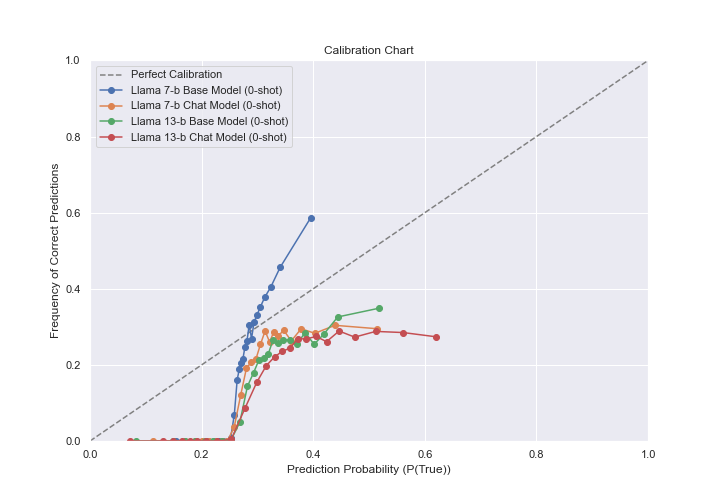
\includegraphics[width=1.1\textwidth]{figures/0-shot-MMLU.png}
         \caption{\textbf{0-shot MMLU} }
         \label{fig:0-shot-MMLU}
     \end{subfigure}
     \hfill
         \begin{subfigure}[b]{0.38\textwidth}
         \centering 
         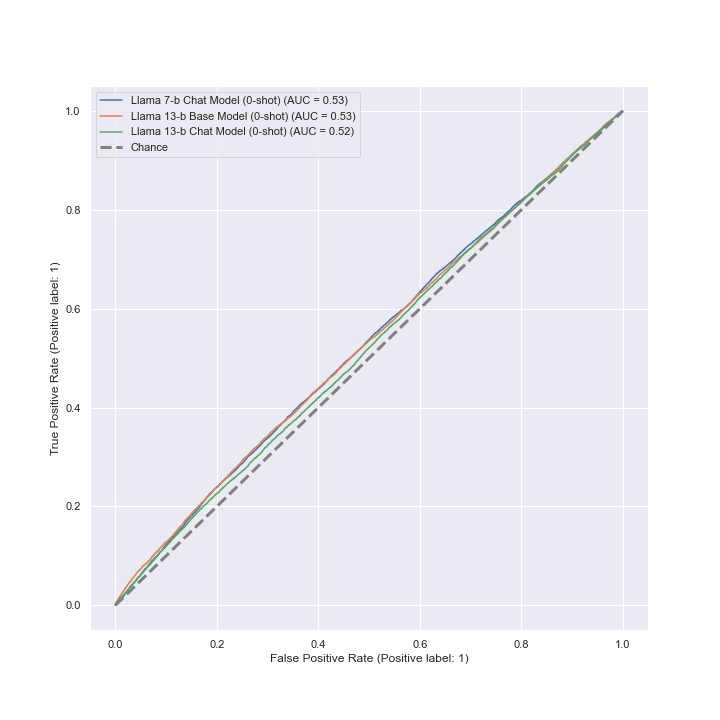
\includegraphics[width=0.9\textwidth]{figures/0-shot-MMLU-roc.png}
         \caption{\textbf{0-shot MMLU ROC}}
         \label{fig:0-shot-MMLU}
    \end{subfigure}  
     \hfill
     \begin{subfigure}[b]{0.60\textwidth}
         \centering
         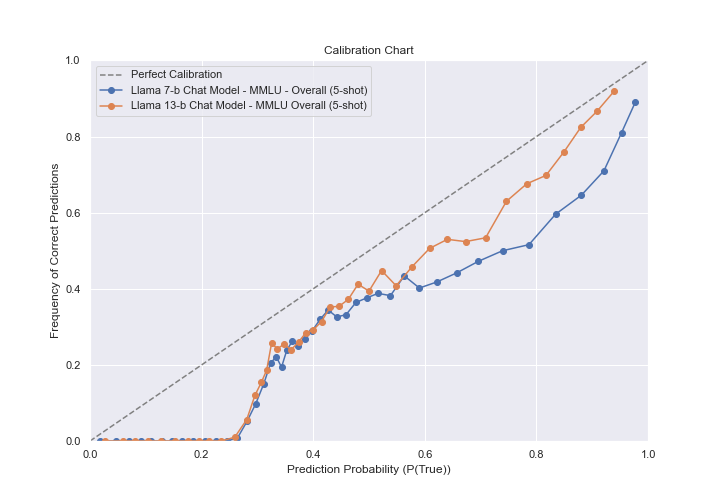
\includegraphics[width=1.1\textwidth]{figures/5-shot-MMLU.png}
         \caption{\textbf{5-shot MMLU} }
         \label{fig:5-shot-logicqa}
     \end{subfigure}     
     \begin{subfigure}[b]{0.38\textwidth}
         \centering 
         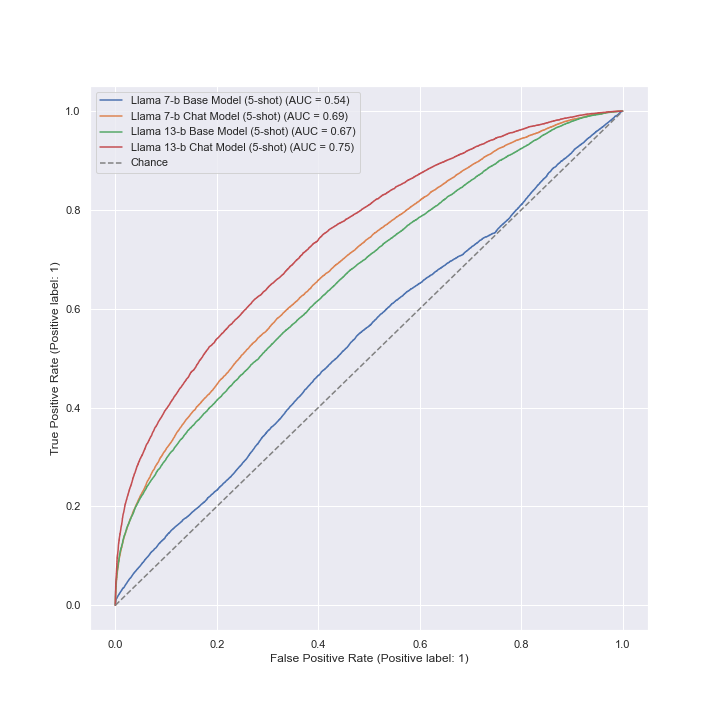
\includegraphics[width=0.9\textwidth]{figures/5-shot-MMLU-roc.png}
         \caption{\textbf{5-shot MMLU ROC} }
         \label{fig:0-shot-MMLU}
    \end{subfigure} 
    
        \caption{\textbf{Calibration and Accuracy on MMLU Dataset:}. We note that few-shot prompting leads to greater accuracy and calibration for fine-tuned chat models. Without fine-tuning base models under-predict their selecting the correct answer. The AUROC curves for base models is greater than those for corresponding fine-tuned models under 0-shot prompting. However in few-shot prompting fine-tuned models perform bbetter than base models in both calibration and accuracy. Additionally a sufficiently large chat model for example 70b chat model is able to display good calibration regardless of few-shot prompting.}
        
        \label{fig:three graphs}
\end{figure*}

\begin{figure*}
     \centering
     \begin{subfigure}[b]{0.60\textwidth}
         \centering 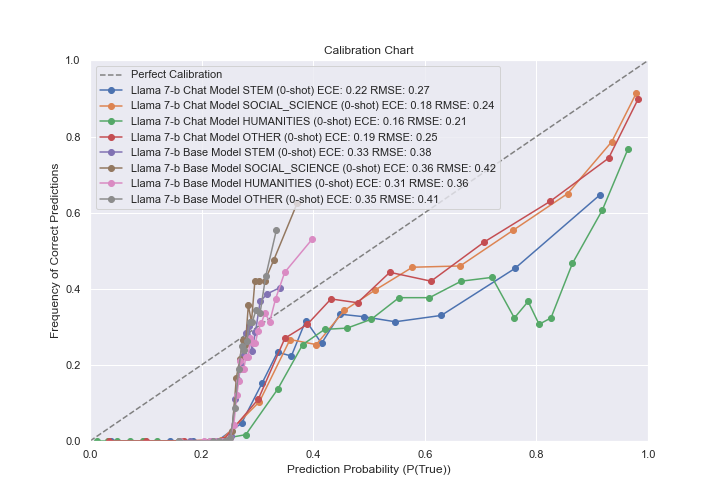
\includegraphics[width=1.1\textwidth]{figures/0-shot-MMLU-subjects-7b.png}
         \caption{\textbf{0-shot MMLU by Subject(7b):} }
         \label{fig:0-shot-MMLU}
     \end{subfigure}
     \hfill
     \begin{subfigure}[b]{0.38\textwidth}
         \centering 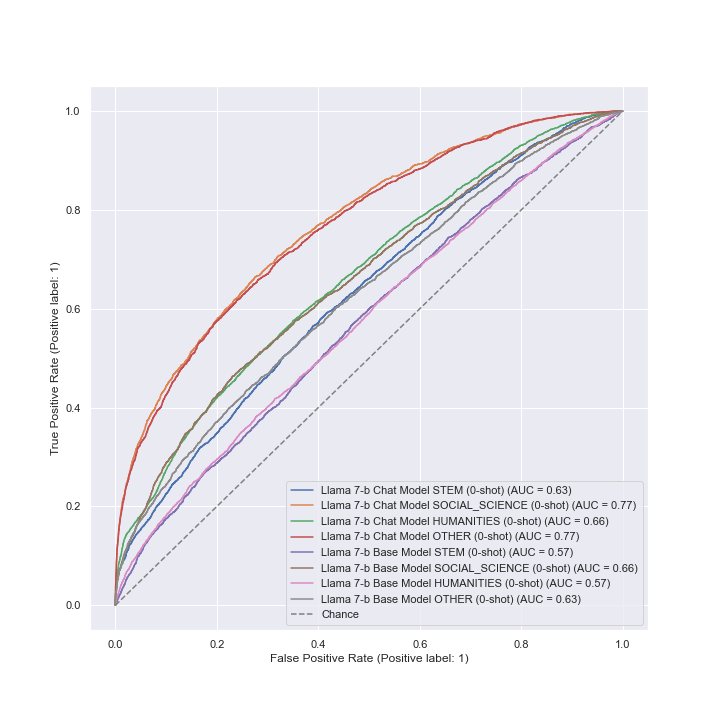
\includegraphics[width=0.9\textwidth]{figures/0-shot-MMLU-subjects-7b-roc.png}
         \caption{\textbf{0-shot MMLU by Subject ROC (7b):} Performance on MMLU shows poor classification, however few-shot prompting enhances classification for subjects the model is predisposed to answer}
         \label{fig:0-shot-MMLU-ROC}
    \end{subfigure}
    
     \hfill
     \begin{subfigure}[b]{0.60\textwidth}
         \centering
         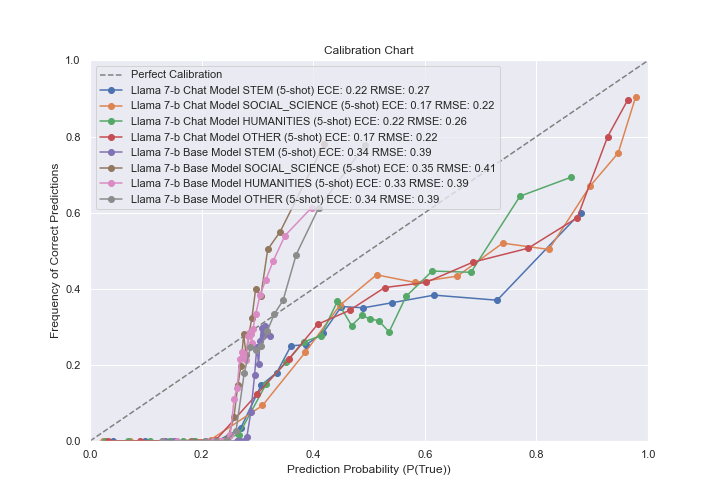
\includegraphics[width=1.1\textwidth]{figures/5-shot-MMLU-subjects-7b.png}
         \caption{\textbf{5-shot MMLU by Subject(7b):}  For subjects which the model can correctly 
         answer few-shot prompting improves accuracy and calibration}
         \label{fig:5-shot-logicqa}
     \end{subfigure}     
    \hfill 
     \begin{subfigure}[b]{0.38\textwidth}
         \centering 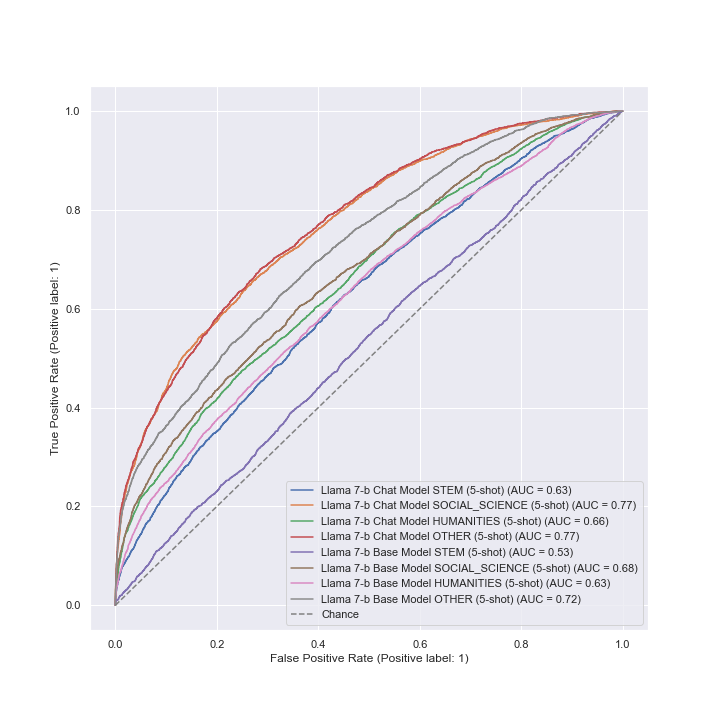
\includegraphics[width=0.9\textwidth]{figures/5-shot-MMLU-subjects-7b-roc.png}
         \caption{\textbf{5-shot MMLU by Subject ROC (7b):} We note large increase in accuracy for 
         Humanities and Other, category with few-shot prompting}
         \label{fig:0-shot-MMLU}
    \end{subfigure} 
    
        \caption{Calibration Performance of Chat and Base models on the MMLU multiple choice question answering dataset.}
        \label{fig:three graphs}
\end{figure*}

\begin{figure*}
     \centering
     \begin{subfigure}[b]{0.60\textwidth}
         \centering 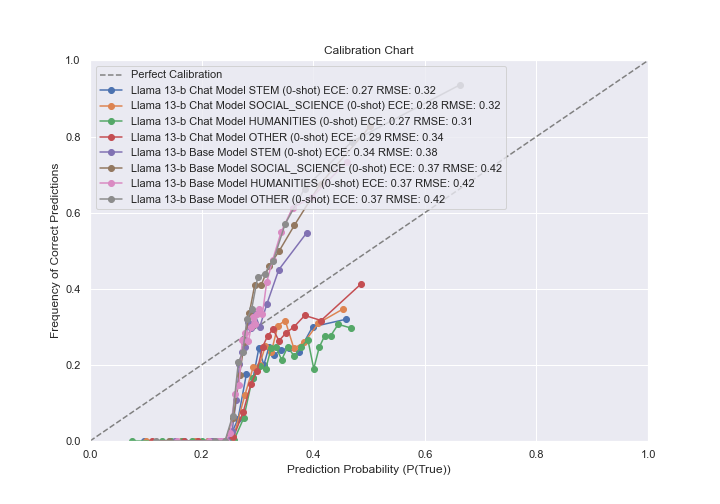
\includegraphics[width=1.1\textwidth]{figures/0-shot-MMLU-subjects-13b.png}
         \caption{\textbf{0-shot MMLU by Subject(13b):}  Base models out perform fine-tuned models, but they are not calibrated and predict lower probabilities for correct answers}
         \label{fig:0-shot-MMLU}
     \end{subfigure}
     \hfill
     \begin{subfigure}[b]{0.38\textwidth}
         \centering 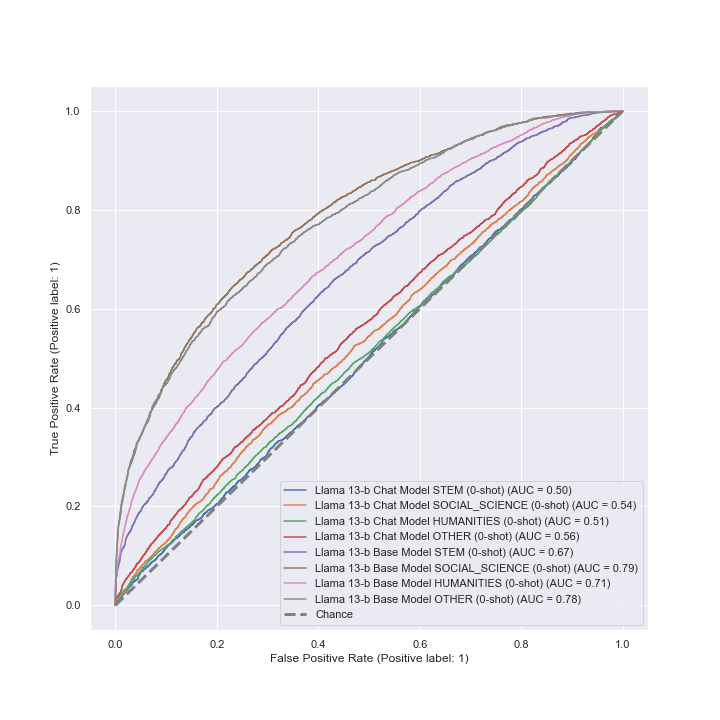
\includegraphics[width=0.9\textwidth]{figures/0-shot-MMLU-subjects-13b-roc.png}
         \caption{\textbf{0-shot MMLU by Subject ROC (13b):} Performance on MMLU shows poor classification, however few-shot prompting enhances classification for subjects the model is predisposed to answer}
         \label{fig:0-shot-MMLU-ROC}
    \end{subfigure}
    
     \hfill
     \begin{subfigure}[b]{0.60\textwidth}
         \centering
         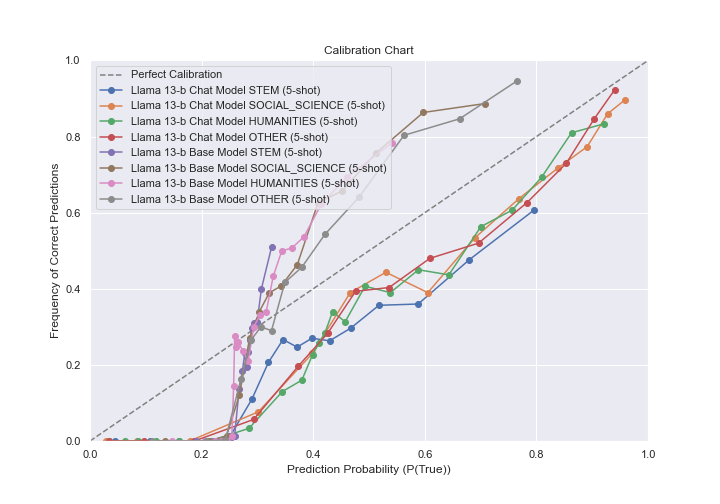
\includegraphics[width=1.1\textwidth]{figures/5-shot-MMLU-subjects-13b.png}
         \caption{\textbf{5-shot MMLU by Subject(13b):}  For subjects which the model can correctly 
         answer few-shot prompting improves accuracy and calibration}
         \label{fig:5-shot-logicqa}
     \end{subfigure}     
    \hfill 
     \begin{subfigure}[b]{0.38\textwidth}
         \centering 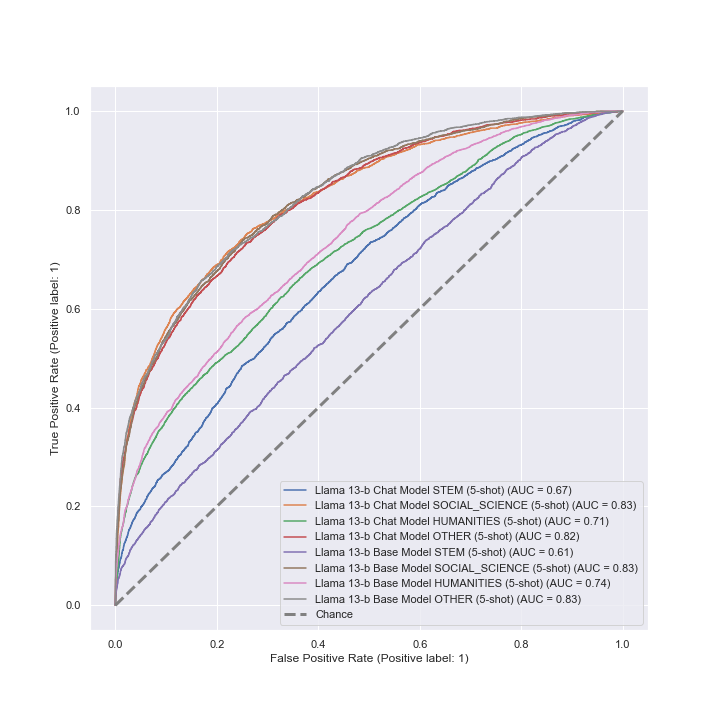
\includegraphics[width=0.9\textwidth]{figures/5-shot-MMLU-subjects-13b-roc.png}
         \caption{\textbf{5-shot MMLU by Subject ROC (13b):} We note large increase in accuracy for 
         Humanities and Other, category with few-shot prompting}
         \label{fig:0-shot-MMLU}
    \end{subfigure} 
    
        \caption{Calibration Performance of Chat and Base models on the MMLU multiple choice question answering dataset.}
        \label{fig:three graphs}
\end{figure*}
\
\subsection{Model Calibration By Number of Parameters}

We compare the calibration of the Llama \cite{touvron2023llama} model 
7b-chat and 13b chat models for answering multiple choice questions in 
figure ... 

We note that that the calibration of the model while not perfect improves with the size of the model with the 13b-chat model being better calibrated and closer to the ideal calibration line than the 7b-chat model. Thus we  note that models sizes improves not only the performance of the model but the calibration of the model as well.

\begin{figure*}
     \centering
     \begin{subfigure}[b]{0.60\textwidth}
         \centering 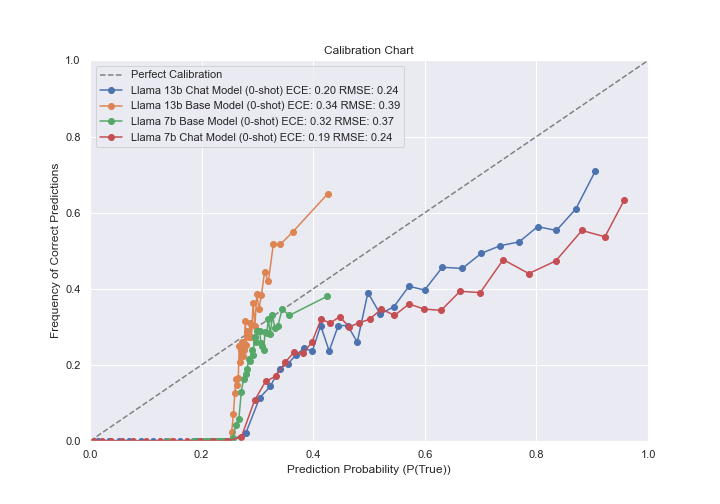
\includegraphics[width=1.0\textwidth]{figures/0-shot-logic-qa.png}
         \caption{\textbf{0-shot Logic QA:} We note the base model under-predicts its performance.} 
         \label{fig:0-shot-MMLU}
     \end{subfigure}
     \hfill
     \begin{subfigure}[b]{0.38\textwidth}
         \centering 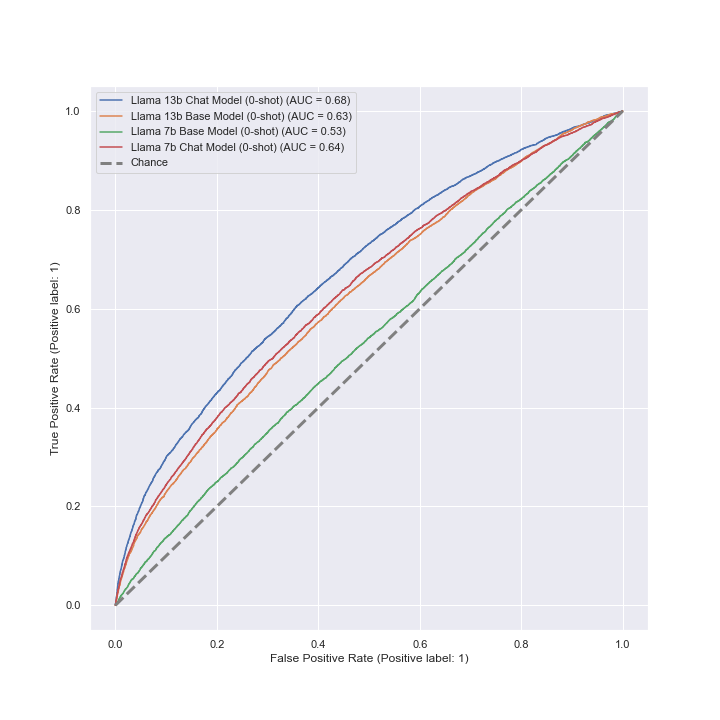
\includegraphics[width=0.9\textwidth]{figures/0-shot-logic-qa-roc.png}
         \caption{\textbf{0-shot Logic QA ROC:} Bigger fine-tuned modes better accuracy},
         \label{fig:0-shot-MMLU}
    \end{subfigure}  
    
     \hfill
     \begin{subfigure}[b]{0.60\textwidth}
         \centering
         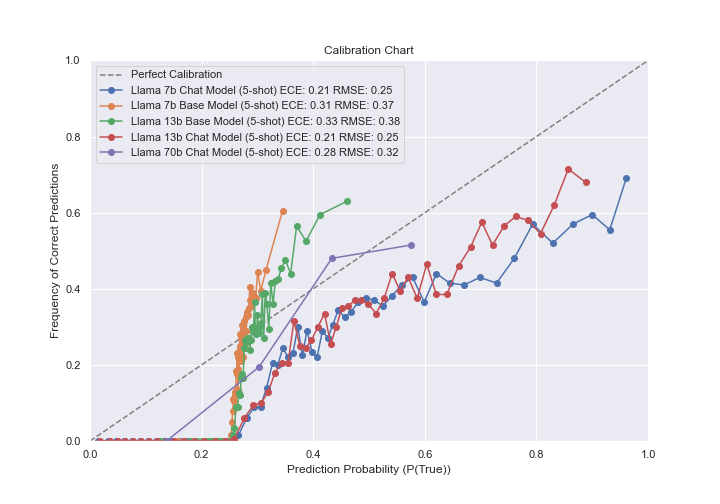
\includegraphics[width=1.0\textwidth]{figures/5-shot-logic-qa.png}
         \caption{\textbf{5-shot Logic QA:} Chat models improve in calibration in 5-shot model, much like MMLU. Base models do not show any such improvement.}
         \label{fig:5-shot-logicqa}
     \end{subfigure}     
    \hfill 
     \begin{subfigure}[b]{0.38\textwidth}
         \centering 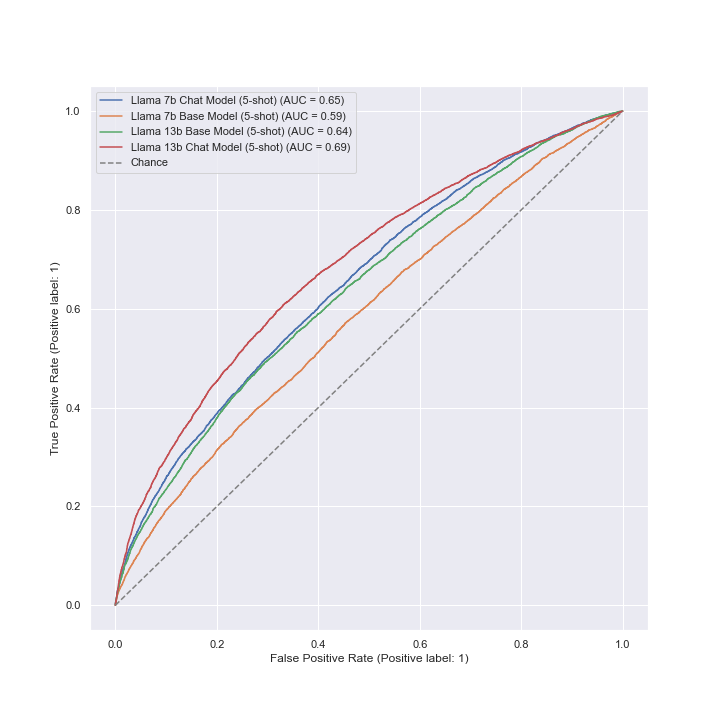
\includegraphics[width=0.9\textwidth]{figures/5-shot-logic-qa-roc.png}
         \caption{\textbf{5-shot Logic QA ROC:}  note that we do not see significant differences in performance before and after prompting. Fine tuning however improves performance and calibration},
         \label{fig:0-shot-MMLU}
    \end{subfigure} 
     
     
        \caption{Calibration Performance of Chat and Base models on the LogicQA , logical question answering dataset}
        \label{fig:three graphs}
\end{figure*}

\begin{figure*}
     \centering
     \begin{subfigure}[b]{0.60\textwidth}
         \centering 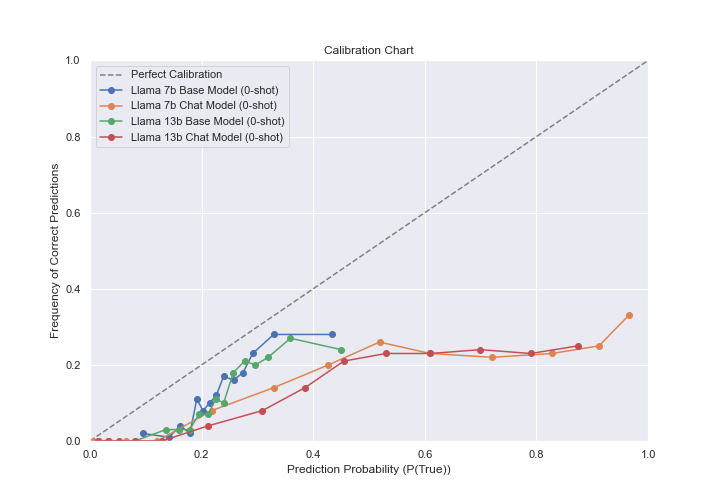
\includegraphics[width=1.0\textwidth]{figures/0-shot-truthful_qa.png}
         \caption{\textbf{0-Shot TruthfulQA:} We note that chat models suffer from overconfidence in 0-shot models, moreover model size fails to show significant improvement on TruthfulQA dataset}
         \label{fig:0-shot-truthfulqa}
     \end{subfigure}
     \hfill
     \begin{subfigure}[b]{0.38\textwidth}
         \centering 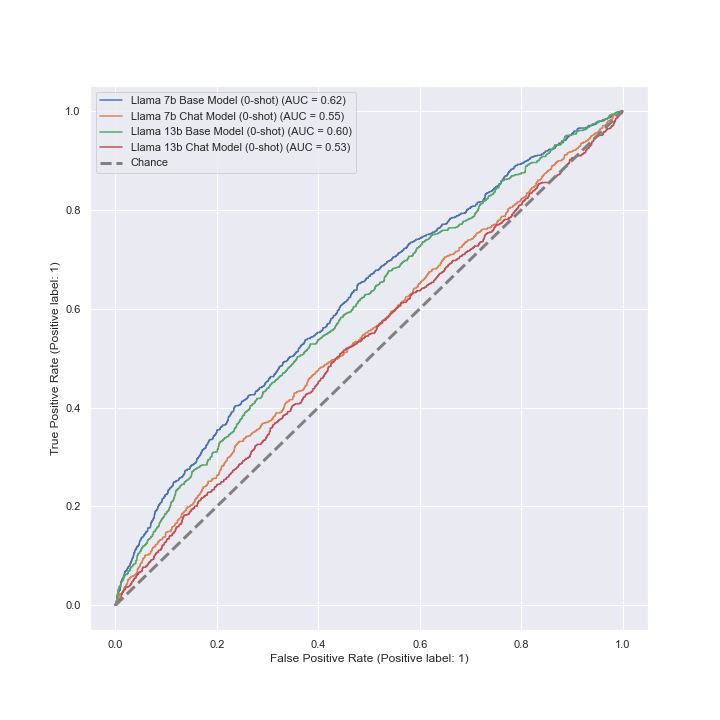
\includegraphics[width=0.9\textwidth]{figures/0-shot-truthful_qa-roc-roc.png}
         \caption{\textbf{0-shot TruthfulQA:} Base models marginally outperform fine-tuned chat models 
         in terms of accuracy},
         \label{fig:0-shot-MMLU}
    \end{subfigure} 
     \hfill
     \begin{subfigure}[b]{0.60\textwidth}
         \centering
         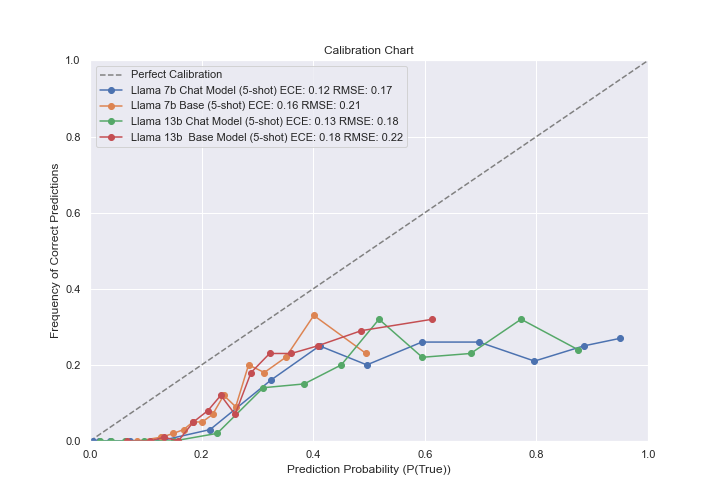
\includegraphics[width=1.0\textwidth]{figures/5-shot-TruthQA.png}
         \caption{\textbf{5-shot Truthful QA:} Truthful QA finds chat models overconfident in their prediction after fine-tuning. No large increase in accuracy or calibration is observed.}
         \label{fig:5-shot-truthfulqa}
     \end{subfigure}    
     \hfill
    \begin{subfigure}[b]{0.38\textwidth}
         \centering 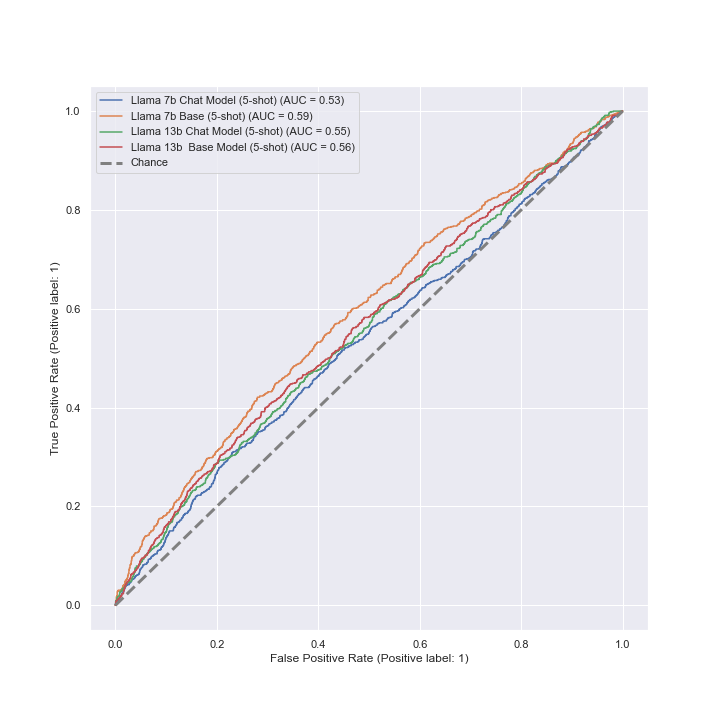
\includegraphics[width=0.9\textwidth]{figures/5-shot-TruthfulQA-roc.png}
         \caption{\textbf{5-shot Truthful QA:}  Multiple shot prompting worsens performance of fine-tuned models},
         \label{fig:0-shot-MMLU}
    \end{subfigure} 
        \caption{Calibration Performance of Chat and Base models on the Truthful QA , logical question answering dataset}
        \label{fig:three graphs}
\end{figure*}



\subsection{Model Calibration By Fine Tuning}  

We first note that fine tuning improves 0-shot calibration. For both 7b and 13b models as observed in 
Figure: \ref{fig:chat-vs-hf}. Where we note the chat model is closer to the ideal calibration line. Moreover we observe that 
few-shot prompting as substantially improves the calibration of smaller 7-b model bringing it closer to calibration performance 13-b model used without prompting.


\subsection{Model Calibration By Subject Specialization}  

Another interesting phenomenon is seen for subject specialization on the MMLU bench mark. We note that calibration for 13b models  trends closer to ideal calibration line for more confident response with the exception of STEM fields where the calibration is substantially worse, having us conclude that the model 
is overconfident and incorrect on scientific questions.



\FloatBarrier

\subsection{HumanEval}

\begin{figure}
  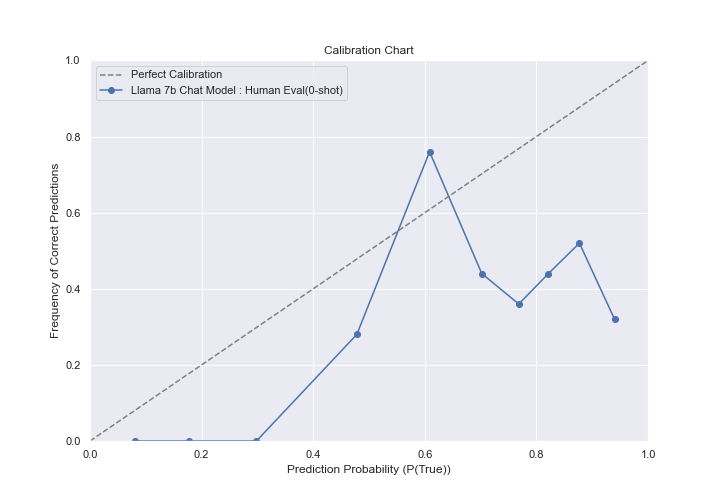
\includegraphics[width=0.5\textwidth]{figures/0-shot-7b-human-eval.png}
  \caption{We run a boolean model, to asses ability of model to judge if a proposed solution satisfies a requirement on human eval dataset.}
  \label{fig:human-eval-results}
\end{figure}

\subsection{GSM8k}

\subsection{Trivia QA}


\section{Discussion}
%%  Discussion: reflection on the results in light of the 
%% research question, discussion of limitations of the current 
%% study and possible future directions for research. 
%% What worked, what didn’t (why, if you have ideas)? 
%% This could include ideas that you had during the 
%% project that you think would be interesting to explore.


\section{Conclusion}
%% Conclusion (optional, could be combined with the discussion)

In this study we attempted to study language model calibration  under various conditions such as model size, fine tuning and task specialization. We find that we were able to replicate the observed  calibration behavior of closed source models like 
GPT-3, and  Claude on the open models like Llama base and fine-tuned chat variants. 

On LogicQA, MMLU datasets we find that fine-tuned chat models are better calibrated than their base variants.
We find that these fine-tuned chat models respond very well to few-shot prompting, with their accuracy and and calibration improving significantly from 0-shot to 5-shot prompting. Additionally simply increasing 
model size going from 7b to 13b to 70b increases model's accuracy and calibration. Inside of MMLU dataset we find  STEM dataset remains hardest in terms both accuracy and calibration though we do see improvements with larger model sizes.

On difficult datasets such as TruthfulQA, where the 
model is not able to attain high accuracy, fine-tuning 
increase model's confidence without the corresponding 
increase in accuracy. This leads us to believe that 
calibration is fundamentally limited by model 
expressiveness for some subset of questions. Here 
the model cannot, \emph{know that it doesn't know}. Other strategies apart from model conversational 
fine-tuning are thus required to increase model calibration in these datasets.

\section{Acknowledgements}

%% Acknowledgments (optional, should be used to 
%% acknowledge collaboration with other groups or, e.g., 
%% usage of coding & writing assistants, other people’s code etc.)

\section{References}

The software to generate and reproduce the study 
along with the gathered data is publicly available at \cite{Nair_Examining_Calibration_Large}.   

%% logicqa  - liu2020logiqa
%% thruthfulqa  - lin2021truthfulqa
%% mmlu - hendryckstest2021 
%% MMLU  - hendrycks2021ethics
%% GSM8K - cobbe2021gsm8k
%% trivia-qa - 2017arXivtriviaqa
%% humaneval - chen2021evaluating

% Entries for the entire Anthology, followed by custom entries
\bibliography{anthology,custom}
\bibliographystyle{acl_natbib}
\appendix
\section{Appendix}

\subsection{Study Materials}

\label{sec:appendix}

\end{document}
